\documentclass{article}

%\usepackage{graphicx}

%\usepackage{amsmath}

\usepackage{gvv-book}

\usepackage{gvv}

%\usepackage{float}

\usepackage{enumitem}

%\usepackage{tfrupee}

%\title{CBSE}

%\usepackage{romannum}

%\date{september 2024}

\begin{document}

\begin{enumerate}

\item A man standing on the deck of a ship,which is $10 m$ above water level, observes the angle of elevation of the top of a hill as $60^{\degree}$ and the angle of depression of the base of hill as $30^{\degree}$. Find the distance of the hill from the ship and the height of the hill.

\end{enumerate}
\end{document}
\item In \figref{fig:twocircle}, two equal circles,with centres $O$ and $O'$, touch each other at $X$.$OO'$ produced meets the circle with centre $O'$ at $A$. $AC$ is tangent to the circle with centre $O$, at the point $C$. $O'D$ os perpendicular to $AC$. Find the value of $\frac{DO'}{CO}$.                                       \begin{figure}[H]                         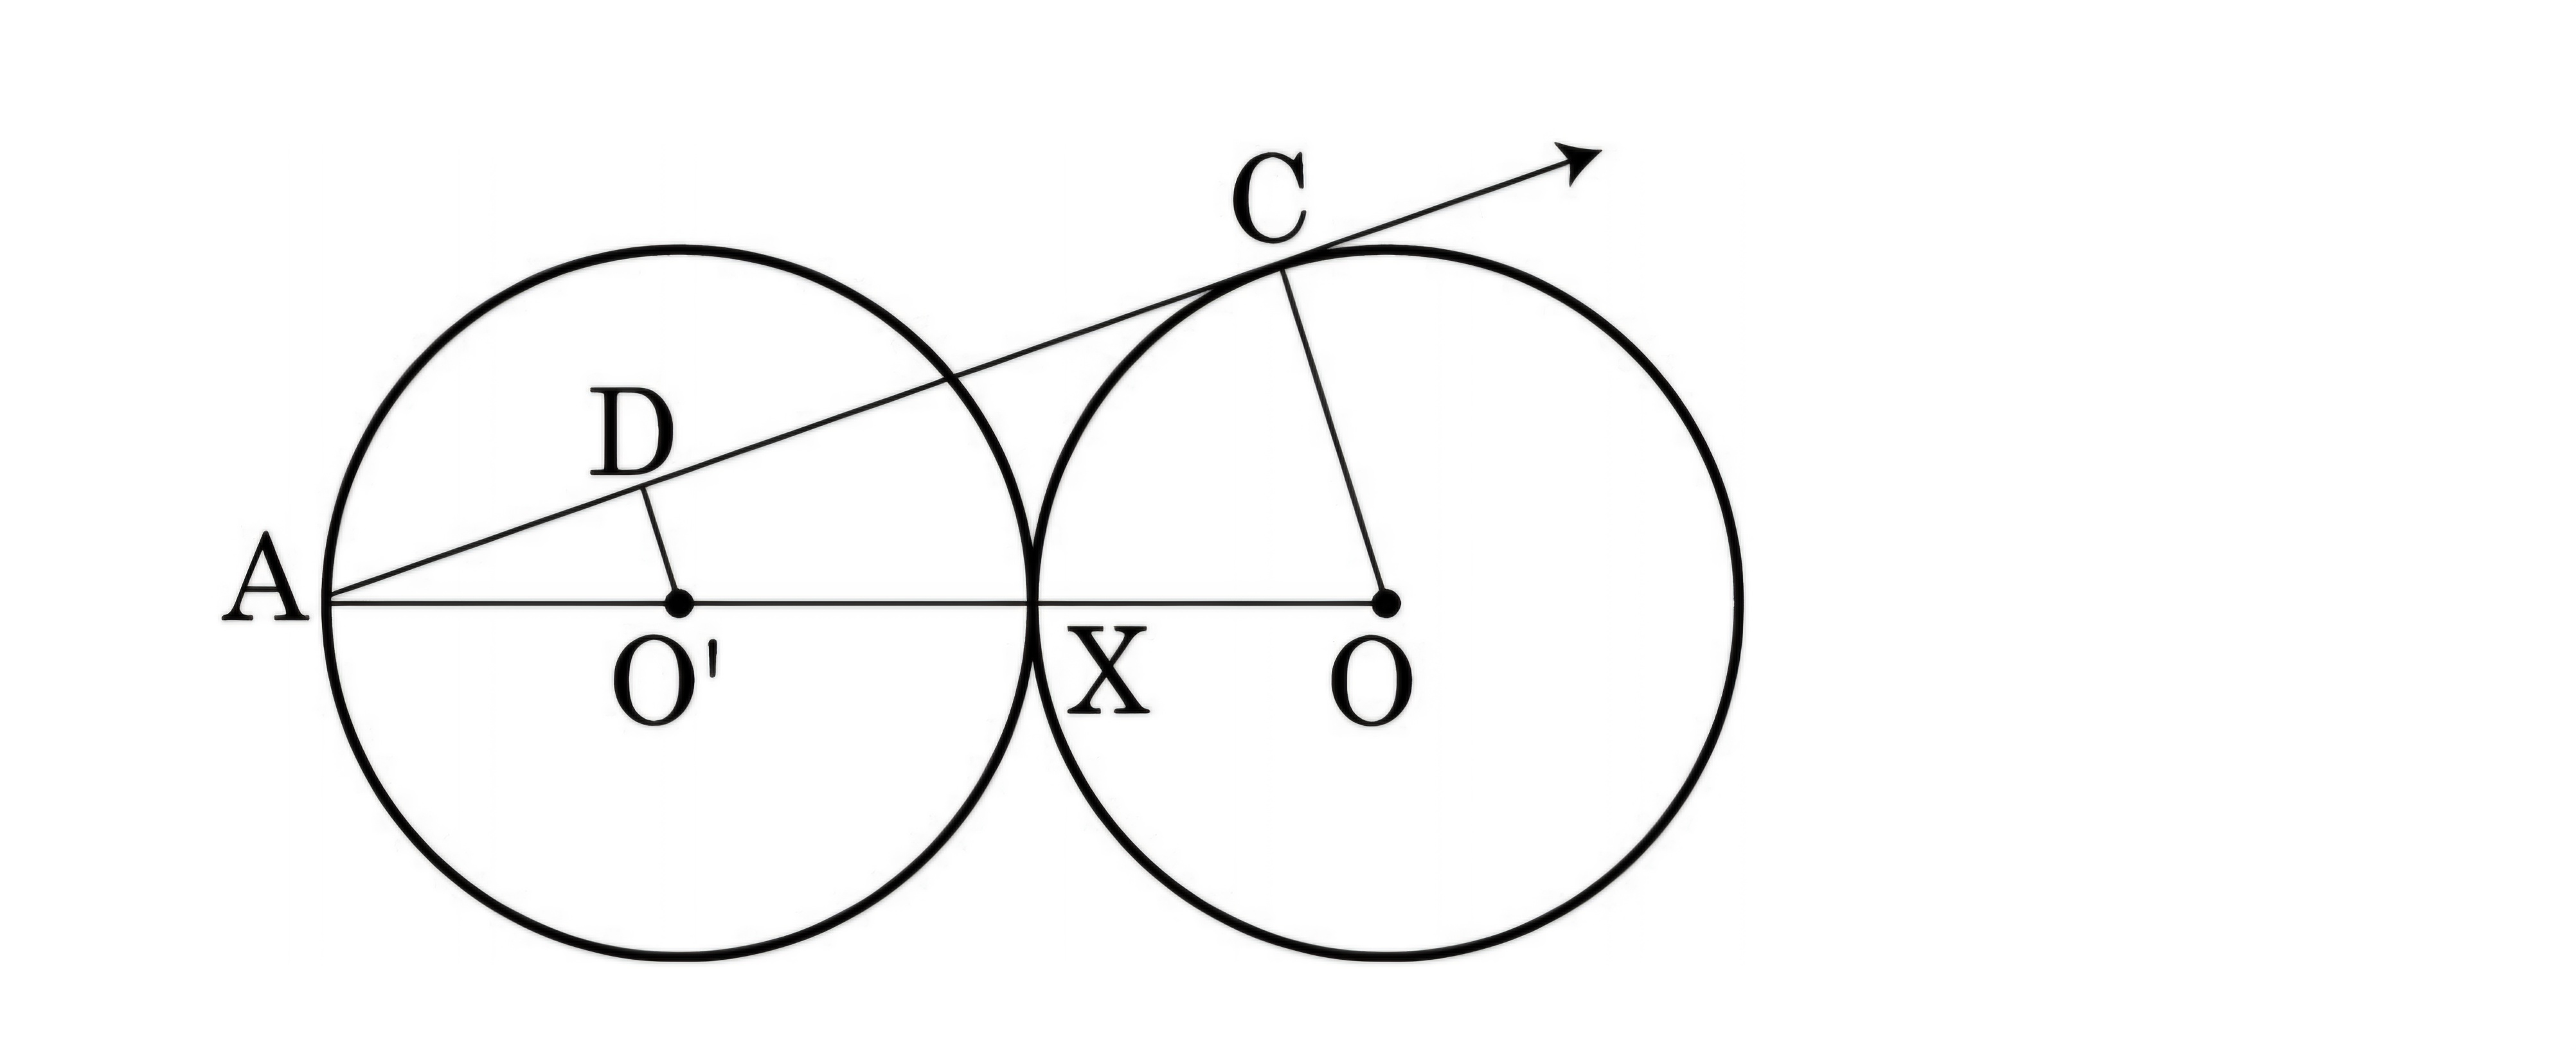
\includegraphics[width=\columnwidth]{./figs/twocircle.jpg}                         \caption{Two equal circles}               \label{fig:twocircle}                    \end{figure}                        \item solve for $x$ :                            \begin{align}                                    \frac{1}{x+1}+\frac{2}{x+2}=\frac{4}{x+4},x \not=-1,-2,-4                 \end{align}
		\end{enumerate}
		\end{document}
